\subsection{Dopremanje namirnica}
\begin{figure}[H]
\begin{center}
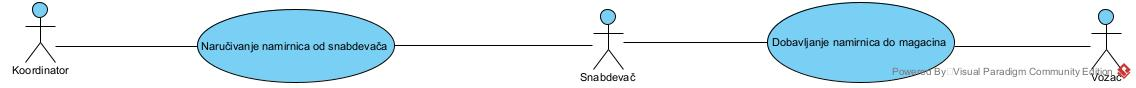
\includegraphics[width=\textwidth]{uc_diagram_groceries_supply.jpg}

    \caption{Dijagram slučaja nabavke namirnica}
    \end{center}
\label{fig:Uc_diagram_groceries_supply}
\end{figure}

Na slici \ref{fig:bpmnGroceryDelivery} je prikazan BPMN dijagram saradnje i on predstavlja sled događaja u sistemu za slučajeve upotrebe: 
\begin{itemize}
	\item{Naručivanje namirnica od snabdevača}
	\item{Prijem i rapoređivanje dostiglih namirnica}
\end{itemize}

Koordinator proverava u sistemu koje namirnice fale i naručuje ih od snabdevača.
Poručivanje se vrši preko sistema. Magacioner prima narudžbine i beleži u sistemu sta je dopremljeno.


\begin{figure}[H]
	\begin{center}
		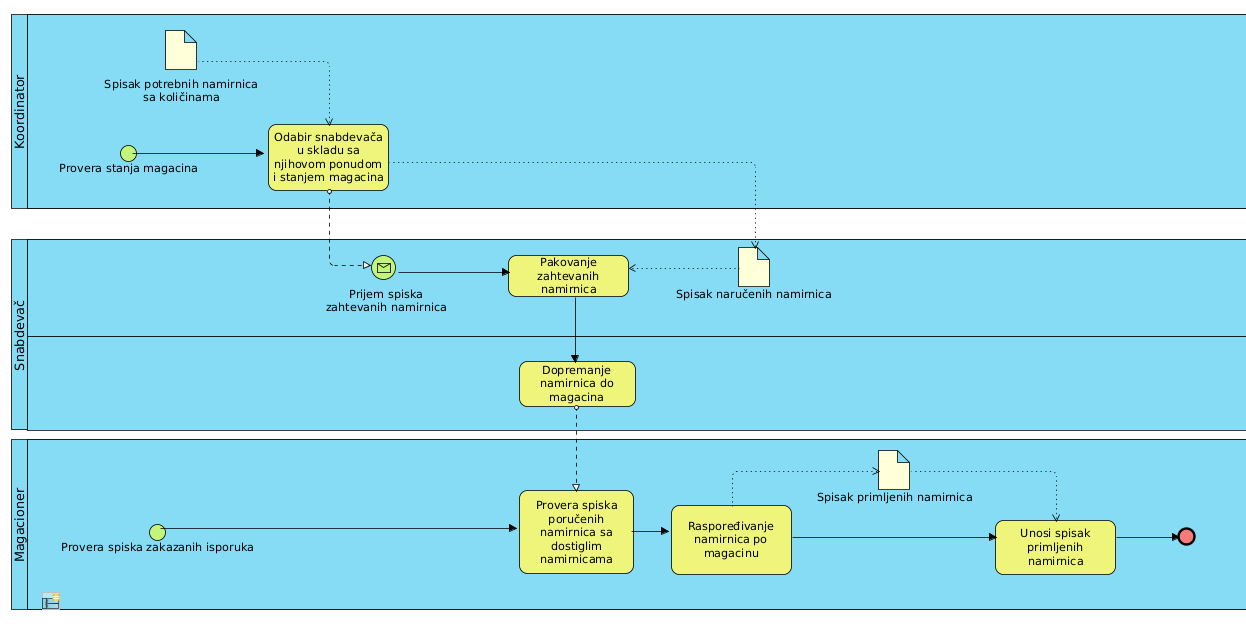
\includegraphics[width=\textwidth]{Pictures/bpmn_grocery_delivery.png}
	\end{center}
    \caption{BPMN dijagram saradnje dopremanja namirnica}
\label{fig:bpmnGroceryDelivery}
\end{figure}




\subsubsection{Naručivanje namirnica od snabdevača}


\begin{itemize}
	\item Kratak opis:
		\begin{itemize}
			\item Koordinator proverava status potrebnih namirnica i dogovara narudžbine sa snabdevačima.
		\end{itemize}
	\item Učesnici:
		\begin{itemize}
		    \item Koordinator
		\end{itemize}
	\item Preduslovi:
		\begin{itemize}
		   
		    \item Sistem je u funkciji.
		\end{itemize}
	\item Postuslovi:
		\begin{itemize}
			\item Tražene namirnice su poslate.
	\end{itemize}
	\item Osnovni tok:
		\begin{enumerate}
		  % Sistem je sam izracunao za njega sta tacno fali po narudzbinama koje su korisnici izabrali. Onaj slucaj upotrebe koji vrsi magacioner kad stignu namirnice i sistem kad izracuna pokriva pravljenje spiska stvari koje nedostaju
            \item Koordinator pristupa sistemu i bira opciju za proveru stanja namirnica.
           \item Sistem prikazuje koje namirnice nedostaju i količinu koju treba naručiti.
           \item Koordinator bira opciju pretraživanja ponude snabdevača i bira nedostajuće namirnice.
            \item Sistem prikazuje snabdevača čija ponuda pokriva nedostajuće namirnice. 
             \item  Koordinator selektuje snabdevača i unosi porudžbinu namirnica.
              \item Sistem čuva porudžbinu u bazi.
             \item Sistem šalje obaveštenje snabdevaču sa detaljima narudžbine koju treba da pošalje.
            
            
		\end{enumerate}
		\textit{Koraci 3-7 se ponavljaju dokle god postoje namirnice koje nedostaju a nisu poručene.}
	\item Alternativni tok:
		\begin{itemize}
		    \item[2.a] Ukoliko su sve potrebne namirnice dostupne u magacinu slučaj upotrebe se završava .
		 
		\end{itemize}
   \item Dodatne informacije:
		\begin{itemize}
		    \item Podaci o porudžbini podrazumevaju sve namirnice koje su naručene, njihovu količinu, ime snabdevača koji ih dostavlja i vreme isporuke.
	
		\end{itemize}
\end{itemize}

\begin{figure}[H]
\begin{center}
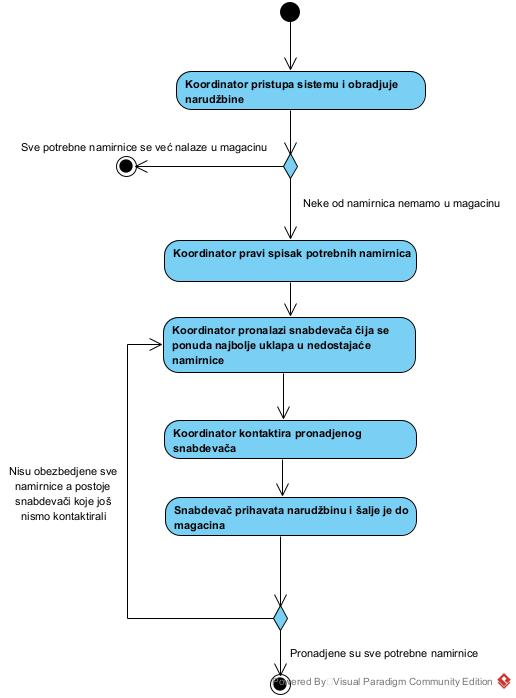
\includegraphics[width=\textwidth]{activity_diagram_order_placment_for_groceries.jpg}
\end{center}
    \caption{Dijagram aktivnosti - Naručivanje namirnica od snabdevača}
\label{fig:Activity_diagram_order_placment_for_groceries}
\end{figure}


\subsubsection{Prijem i rapoređivanje dostiglih namirnica}

	\begin{itemize}
		\item{Kratak opis:} 
		\begin{itemize}
			\item{Magacioner prihvata dostigle namirnice i raspoređuje ih u magacinu}
		\end{itemize}
		\item{Učesnici:} 
		\begin{itemize}
			\item{Magacioner}
		\end{itemize}		
		
		\item{Preduslovi:}
		\begin{itemize}
			\item{Magacioner je prijavljen na sistem.}
		\end{itemize}
		
		\item{Postuslovi:}
		\begin{itemize}
			\item{Sve dostigle namirnice su raspoređene u magacinu i baza podataka je ažurirana.}
		\end{itemize}
		
		\item{Osnovni tok:}
		\begin{enumerate}
			\item{Sistem obaveštava magacionera da je došlo do izmene spiska zakazanih isporuka.}
			\item{Magacioner proverava spisak zakazanih isporuka.}
			\item{Kamion sa poručenim namirnicama dolazi do magacina.}
			\item{Magacioner proverava spisak dostiglih namirnica i njihovu količinu sa listom poručenih namirnica.}
			\item{Magacioner raspoređuje namirnice po magacinu.}
			\item{Magacioner beleži u sistemu da je završen prijem namirnica i spisak primljenih namirnica.}
			\item{Sistem ažurira bazu podataka u skladu sa spiskom primljenih namirnica.}
		\end{enumerate}
		
		\item{Alternativni tok:}
			\begin{enumerate}
				\item[4.a] {Magacioner vrši evidenciju namirnica koje se ne poklapaju na spiskovima i kako se ne poklapaju.} 
				\item[4.b]{Magacioner preuzima samo namirnice koje se poklapaju na spiskovima i u potrebnoj količini ili manjoj.}
			\end{enumerate}
		\item{Dodatne informacije}
			\begin{itemize}
				\item{Informacije o datumu i vremenu isporuke, koji od snabdevača isporučuje namirnice, koje i u kojoj količini, se nalaze na spisku zakazanih isporuka za svaku od planiranih isporuka.}
			\end{itemize}
	\end{itemize}
\begin{figure}[H]
	\begin{center}
		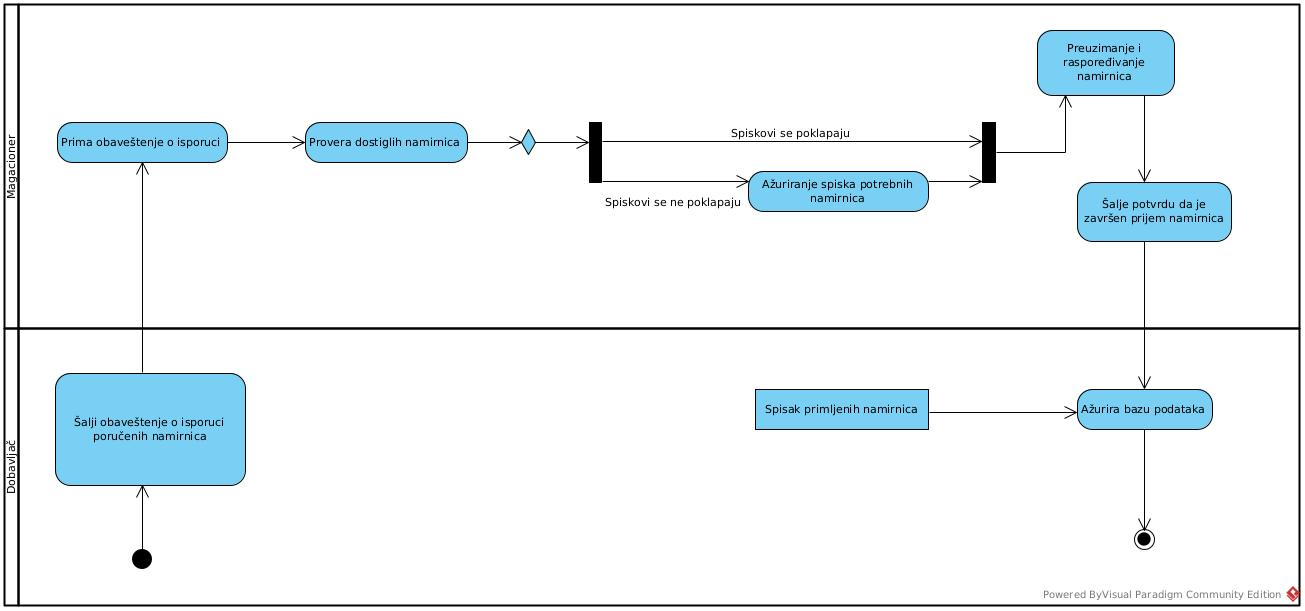
\includegraphics[width=\textwidth]{activity_receiving_groceries}
		\caption{Dijagram aktivnosti prijema i raspoređivanja dostiglih namirnica}
	\end{center}
\end{figure}

